\documentclass{beamer}

\usepackage[T1]{fontenc}
\usepackage[utf8]{inputenc}
\usepackage{lmodern}
\usepackage[english]{babel}
\usepackage{pgfplots}
\pgfplotsset{compat=1.9}
\usepackage{booktabs}
\usepackage{siunitx}

\usepackage{subfig}
\usetikzlibrary{arrows,decorations.pathmorphing,fit,positioning}

\setbeamerfont{note page}{size=\footnotesize}
%\setbeameroption{show only notes}

\usetheme[department=compute]{DTU}

\title{Opinion Spam Detection Through Semantic Similarity}
\author{Vlad Sandulescu}
%\institute{\LaTeX\ Support Group, Technical University of Denmark (DTU)}

\newcommand{\tabitem}{{\color{dtured}$\bullet$} }

\begin{document}
\frame{
	\maketitle
}

\frame{
	\frametitle{Outline}
	\tableofcontents
}

\section{Introduction}
\subsection{Problem}
\frame{
	\frametitle{Online reviews}

		\begin{center}

			\includegraphics[height=1cm,keepaspectratio]{fig/tripadvisor.jpg} \, \includegraphics[height=1.4cm,keepaspectratio]{fig/yelp.jpg}
			\vspace{.5cm}
			\includegraphics[height=1cm,keepaspectratio]{fig/amazon.jpg} 
			\vspace{.5cm}
			\includegraphics[height=1cm,keepaspectratio]{fig/trustpilot.jpg} 
			\vspace{.5cm}
			\includegraphics[height=1cm,keepaspectratio]{fig/foursquare.jpg} \,			
\includegraphics[height=1cm,keepaspectratio]{fig/google.jpg} 
			
		\end{center}
		
		\begin{center}
			\begin{itemize}
				\item 31\% of consumers read online reviews before actually making a purchase (rising)
				\item by the end of 2014, 15\% of all social media reviews will consist of company paid fake reviews
			\end{itemize}

		\end{center}

	\note{Online reviews have become in recent years a very important resource for consumers when making purchases. The number of consumers that first read reviews about a product they wish to buy is constantly on the rise. Technology research company Gartner Inc. claims 31\% of consumers read online reviews before actually making a purchase. As consumers increasingly rely on these ratings, the incentive for companies to try to produce fake reviews to boost sales is also increasing. Gartner predicts in 2014 as much as 15 percent of all social media reviews will consist of company paid fake reviews.}
	
}

\subsection{Related Work}
\frame[allowframebreaks]{
	\frametitle{Two main directions: behavioral features and text analysis}
		\begin{center}
			\includegraphics[width=\textwidth,keepaspectratio]{fig/fake_review.png} 
		\end{center}
		
		\begin{center}
			\begin{itemize}
				\item Behavioral approach gives good results for "elite" users 
				\item $\sim$ 90\% of reviewers write a single review
				\item Textual analysis = mostly cosine similarity, but also linguistic cues of deceptive writing - using more verbs, adverbs and pronouns
				\item "husband" or "vacation" = highly suspicious based on their incidence in fake reviews
				\item \textbf{What happens to singleton reviewers?} 
			\end{itemize}

		\end{center}

	\note{The first method so far seems to be more reliable and can be more easily put into practice. It also offers very good results as a standalone method, although the textual features do bring little overall improvement. The linguistic techniques used so far mostly consisted of computing cosine similarity between the contents of the reviews. In a new study, the authors concluded that human judgment used to detect semantic similarity of web document does not correlate well with cosine similarity. 
Other researches used a bag-of-words approach and calculated the frequency of certain words from the review text. They then classified some reviews as suspicious if the text contained a high number of predefined suspicious words. This led to more subjective conclusions that spammers prefer to use more personal pronouns than genuine reviewers or they usually write reviews of more than 150 characters on average. An obvious aspect is that once the spammers find out about these textual frequency traps which cause suspicion, they will simply avoid them.}
}

\subsection{Goals}
\frame{
	\frametitle{Goals and challenges}
	\begin{block}{Hypothesis}
		\begin{itemize}
			\item Semantic similarity measures should outperform vector based models because they should also capture more subtle deception attempts
			\item A spammer's imagination is limited, so he will partially reuse some of the aspects between reviews, through paraphrase and synonyms
		\end{itemize}
	\end{block}

	\begin{block}{Goal}
		\begin{itemize}
			\item Detect opinion spam using semantic similarity (WordNet) and topic modeling (LDA)
			\item Compare the performance to vectorial-based similarity measures (cosine)
		\end{itemize}
	\end{block}

	\note{This thesis proposes a complete solution to detect opinion spam of one-time reviewers using semantic similarity. It also proposes a method to detect opinion spam, using recent research models aimed at extracting product aspects from short texts, based on topic modeling and in particular on Latent Dirichlet Allocation (LDA). Another goal was to test this hypothesis on real-life reviews and make a comparison with the existing vectorial similarity models, which are based on cosine similarity. 

My hypothesis is that semantic similarity measures should outperform vector based models because they should also capture more subtle deception behavior, meaning more paraphrase intent of the spammers. Detecting fake reviews through semantic similarity methods would inherently work on users who operate in groups, know one other and paraphrase or rephrase each other's reviews inside the same group of spammers.}

}


\subsection{Textual Similarity - WordNet}
\frame{
	\frametitle{Textual smilarity}

	\begin{block}{Vectorial-based measures}
	For $T_1$ and $T_2$, their cosine similarity can be formulated as
	\scriptsize
	\begin{equation}
	\cos({ T_1},{ T_2})={{T_1} {T_2} \over \|{ T_1}\| \|{ T_2}\|} = \frac{ \sum_{i=1}^{n}{{ T_1}_i{ T_2}_i} }{ \sqrt{\sum_{i=1}^{n}{({ T_1}_i)^2}} \sqrt{\sum_{i=1}^{n}{({ T_2}_i)^2}} }
	\end{equation}
	\normalsize
	\end{block}

	\begin{block}{Knowledge-based measures}
	For $T_1$ and $T_2$, their semantic similarity (Mihalcea et al.) can be formulated as:
	\scriptsize
	\begin{equation}\label{eq:mihalcea-definition}
	sim({ T_1},{ T_2})=\frac{1}{2}(\frac{\sum\limits_{w\in\{T_1\}}{(maxSim(w,T_2)*idf(w))}}{\sum\limits_{w\in\{T_1\}}{idf(w)}} + \frac{\sum\limits_{w\in\{T_2\}}{(maxSim(w,T_1)*idf(w))}}{\sum\limits_{w\in\{T_2\}}{idf(w)}})
	\end{equation}
	\normalsize
	\end{block}

	\begin{center}
		\textbf{transport} - "The \textbf{shop} now offers \textbf{night} \textbf{delivery}"
	\end{center}

	\note{
Given a metric for word-to-word similarity(WordNet) and a measure of word specificity(idf)(no. of documents in corpus / no. of documents containing the word), we define the semantic similarity of two text segments T1 and T2 using a metric that combines the semantic similarities of each text segment in turn with respect to the other text segment. 

First, for each word w in the segment T1 we try to identify the word in the segment T2 that has the highest semantic similarity (maxSim(w,T2)). Next, the same process is applied to determine the most similar word in T1 starting with words in T2. The word similarities are then weighted is applied to determine the most similar word in T1 starting with words in T2. The word similarities are then weighted with the corresponding word specificity, summed up, and normalized with the length of each text segment. Finally the resulting similarity scores are combined using a simple average. Only nouns and verbs are matched, for adjectives and adverbs - lexical matching is used. 

This means that, for instance, the most similar word to the noun "transport" within the text "The shop now offers night delivery" will be sought among the nouns "shop", "night" and "delivery", and will ignore the words with a different part-of-speech - "offers", "now".}

}

\frame{
	\frametitle{WordNet synsets}

	\begin{figure}
	\centering
	\includegraphics[width=\textwidth]{fig/transport.png}
	\label{transport}
	\end{figure} 

}

\section{Distribution of truthful and deceptive reviews}
\frame{
	\frametitle{Distribution of truthful and deceptive reviews}

	\begin{block}{Do fake reviews have a different similarity distribution compared to the truthful reviews?}
		\begin{itemize}
			\item Trustpilot dataset - 8990 reviews 
			\item Ott dataset - 800 reviews (400 fake obtained through AMT)
			\item Stop words removal, POS tagging (extracted NN, JJ, VB)
		\end{itemize}
	\end{block}
	\begin{block}{Cumulative distribution function}
		\begin{equation}
			CDF_X(x) = \operatorname{P}(X\leq x).
		\end{equation}
		\begin{itemize}
			\item Do the distribution curves of the similarity measures overlap for truthful/fake reviews?
			\item Is there a gap between the two curves? If so, what are its bounds?
		\end{itemize}
	\end{block}
	
	\note{Is there a distributional difference, for both vectorial and semantic similarity measures, between deceptive and truthful reviews inside the Trustpilot dataset as well as in the well known dataset used by Ott. Recall that Ott obtained deceptive reviews using Amazon Mechanical Turk - the turkers had to imagine staying at the specific hotels and write their reviews to sound as credible as possible. 

One research study claims that spammers caught by Yelp's filter seem to have "overdone faking" in their attempt to sound more genuine. In their deceptive reviews, they used words that appeared in genuine reviews almost equally frequent and avoided to reuse the exact same words over and over again in their deceptive reviews. This is exactly the reason why a cosine similarity measure is not enough to catch subtle spammers in real life scenarios, such as Yelp's. 

The CDF gives the probability of a random variable \textit{X}, which has a known probability distribution, to have a value less or equal to \textit{x}. The purpose of the CDF curves of truthful/fake reviews is to check if they overlap or there is a separation margin between the two curves. If indeed there is a gap, it would be interesting to know how big this separation is and what are its bounds.  
}
	 
}

\frame{
	\frametitle{Distribution of truthful and deceptive reviews - Trustpilot}
	
	\begin{columns}[T]
		\begin{column}{0.35\textwidth}
			\begin{center}
				Semantic $\sim$ 10\% diff
				\begin{itemize}
					\item {\color{blue} 40\% reviews $\uparrow$ 0.28}
					\item {\color{red} 40\% reviews $\uparrow$ 0.40}
					\item {\color{blue} 80\% reviews $\uparrow$ 0.43}
					\item {\color{red} 80\% reviews $\uparrow$ 0.52}
				\end{itemize}
				\vspace{.2cm}
				Vectorial $\sim$ 0.2\% diff
				\begin{itemize}
					\item {\color{blue} 40\% reviews $\uparrow$ 0.08}
					\item {\color{red} 40\% reviews $\uparrow$ 0.10}
				\end{itemize}
				\vspace{.2cm}
				Steep jump in vectorial
				\begin{itemize}
					\item {\color{red} 20\%-25\% vectorial $\sim$ 0}
					\item {\color{blue} 20\%-25\% semantic $\uparrow$ 0.32}		
				\end{itemize}
			\end{center}
		\end{column}
		\begin{column}{0.8\textwidth}
		\begin{center}		
			\vspace{-.7cm}
			\scriptsize
			Cumulative percentage of reviews vs. similarity values
			\vspace{-.7cm}
				\begin{figure}
				\captionsetup[subfloat]{position=top,font=scriptsize,captionskip=-1.2pt}
				\subfloat[Subfigure 1 list of figures text][Cos]
				{\includegraphics[width=0.4\textwidth,trim=1cm 1.6cm 1cm 1.6cm,clip]{sweave/sweave-trustpilotcosinecdf}
				\label{fig:cdf_trustpilot_cosine}}
				\subfloat[Subfigure 2 list of figures text][CosNonLem]{
				\includegraphics[width=0.4\textwidth,trim=1cm 1.6cm 1cm 1.6cm,clip]{sweave/sweave-trustpilotcosineposnonlemmatizedcdf}
				\label{fig:cdf_trustpilot_cosineposnonlemmatized}}
				\enskip
				\subfloat[Subfigure 3 list of figures text][CosLem ]{
				\includegraphics[width=0.4\textwidth,trim=1cm 1.6cm 1cm 1.6cm,clip]{sweave/sweave-trustpilotcosineposlemmatizedcdf}
				\label{fig:cdf_trustpilot_cosineposlemmatized}}
				\subfloat[Subfigure 4 list of figures text][Mihalcea]{
				\includegraphics[width=0.4\textwidth,trim=1cm 1.6cm 1cm 1.6cm,clip]{sweave/sweave-trustpilotmihalceacdf}
				\label{fig:cdf_trustpilot_mihalcea}}
				\label{fig:cdf_trustpilot}
	
			\end{figure}	
			\normalsize	
		\end{center}	
		\end{column}
	\end{columns}

	\note{The CDF curves plotted reveal several interesting aspects. They show the amount of content similarity for the truthful/fake reviews taken separately as well as the position and bounds for each type and the gaps between the two curves. Regardless of the type of similarity measure used, i.e. vectorial or semantic, the two distributional curves of truthful and fake reviews are clearly separated. For the truthful reviews (blue color), the curve appears towards the left of the plot, while for the fake reviews (red color) it is more towards the right. This means that for any similarity measure applied, for a fixed cumulative percentage value, its corresponding value \textit{$x_t$} for truthful reviews will be lower than the value for deceptive reviews \textit{$x_d$}. 
This shows that people writing deceptive reviews tend to have a higher semantic similarity between their reviews than the users writing honest reviews, probably because they are the same person under multiple accounts or know each other and work together. The honest users do not influence each other's writing style so much. The spammers are more likely to do that.}

}

\frame{
	\frametitle{Distribution of truthful and deceptive reviews - Ott}

	\setcounter{subfigure}{0}
	\begin{columns}[T]
		\begin{column}{0.35\textwidth}
			\begin{center}
				Semantic $\sim$ 8-10\% diff
				\begin{itemize}
					\item {\color{blue} 40\% reviews $\uparrow$ 0.22}
					\item {\color{red} 40\% reviews $\uparrow$ 0.32}
					\item {\color{blue} 80\% reviews $\uparrow$ 0.38}
					\item {\color{red} 80\% reviews $\uparrow$ 0.44}
				\end{itemize}
				\vspace{.2cm}
				Vectorial $\sim$ 0.2\% diff
				\begin{itemize}
					\item {\color{blue} 40\% reviews $\uparrow$ 0.32}
					\item {\color{red} 40\% reviews $\uparrow$ 0.34}
				\end{itemize}
				\vspace{.3cm}
				Why isn't the semantic gap larger?
			\end{center}
		\end{column}
		\begin{column}{0.8\textwidth}
		\begin{center}		
			\vspace{-.7cm}
			\scriptsize
			Cumulative percentage of reviews vs. similarity values
			\vspace{-.7cm}
				\begin{figure}
				\captionsetup[subfloat]{position=top,font=scriptsize,captionskip=-1.2pt}
				\subfloat[Subfigure 1 list of figures text][Cos]
				{\includegraphics[width=0.4\textwidth,trim=1cm 1.6cm 1cm 1.6cm,clip]{sweave/sweave-ottcosine}
				\label{fig:cdf_ott_cosine}}
				\subfloat[Subfigure 2 list of figures text][CosNonLem]{
				\includegraphics[width=0.4\textwidth,trim=1cm 1.6cm 1cm 1.6cm,clip]{sweave/sweave-ottcosineposnonlemmatized}
				\label{fig:cdf_ott_cosineposnonlemmatized}}
				\qquad
				\subfloat[Subfigure 3 list of figures text][CosLem ]{
				\includegraphics[width=0.4\textwidth,trim=1cm 1.6cm 1cm 1.6cm,clip]{sweave/sweave-ottcosineposlemmatized}
				\label{fig:cdf_ott_cosineposlemmatized}}
				\subfloat[Subfigure 4 list of figures text][Mihalcea]{
				\includegraphics[width=0.4\textwidth,trim=1cm 1.6cm 1cm 1.6cm,clip]{sweave/sweave-ottmihalcea}
				\label{fig:cdf_ott_mihalcea}}
				\label{fig:cdf_ott}
	
			\end{figure}	
			\normalsize	
		\end{center}	
		\end{column}
	\end{columns}

	\note{One obvious question is why isn't this gap larger, especially for the semantic similarity measure, regardless of the dataset? 

One possible explanation might be that reviews from the same seller generally talk pretty much about aspects within a very specific context, which is related to the shop's business area of activity. For example, if the shop is an electronics reseller that offers online ordering, home delivery and customer support for sold items, then the review will probably contain aspects related to website, the delivery speed, customer support, service level, screen, battery, price and so on. It is pretty easy for the spammers to mimic the honest reviews in the sense of mentioning the same key aspects in their reviews.

The dataset of Ott has been created using Amazon Mechanical Turk (AMT), so it is likely the turkers was separate persons and did not know each other. It is a different setup than for the real-life Trustpilot dataset, where the fake reviews are more likely to be written by the same people using multiple accounts on the review platform. }

}

\section{Singleton opinion spam detection}
\frame{
	\frametitle{Singleton opinion spam detection - preprocessing \& feature design}

	\begin{columns}[T]
		\begin{column}{0.7\textwidth}
			Trustpilot dataset:
			\begin{itemize}
				\item 8990 English reviews / 130 sellers / 4 or 5 stars / balanced
				\item min-max normalization => all features in [0, 1]

				\begin{equation}
					x’ = \frac{x -min(x)}{max(x)-min(x)}
				\end{equation}
	
				\item Stanford POS tagger, removed stop words, lemmatization
				\vspace{.4cm}

				\textit{"I am working hard on my master thesis at DTU"}

			\end{itemize}
		\end{column}

		\begin{column}{0.3\textwidth}
			Behavioral features:
			\begin{itemize}
				\item review title
				\item review text
				\item review stars rating
				\item review date
				\item user sign up date
				\item review IP
				\item proxy IP
			\end{itemize} 
		\end{column}
	\end{columns}

	\small
	\vspace{.3cm}

	\textit{I/PRP am/VBP working/VBG hard/RB on/IN my/PRP master/NN thesis/NN at/IN DTU/NNP}

	\vspace{.3cm}

	am$\xrightarrow{lemma}$be, working$\xrightarrow{lemma}$work

	\normalsize

}

\frame{
	\frametitle{Singleton opinion spam detection - clustering}
	
	\begin{columns}[T]
		\begin{column}{0.6\textwidth}
			Clustering: DBSCAN \& OPTICS
			\begin{itemize}
				\item density reachability
				\item reduce comparison complexity
			\end{itemize}
			\footnotesize
			\begin{equation}
			MaxSimilarity = \max\limits_{R_i, R_j\in{C}}(sim\_measure(R_i, R_j))
			\end{equation}
			\normalsize
		\end{column}
		\begin{column}{0.4\textwidth}
			\small
				\textit{minPts $\in$ \{2,3\} \\epsilon $\in$  \{0.05, 0.08, 0.1\}}
			\normalsize
			\includegraphics[height=3.1cm,keepaspectratio]{fig/dbscan.png} 
		\end{column}
	\end{columns}

	Similarity measures (all without stop words):
	\begin{itemize}
		\item cosine similarity with all parts-of-speech tags
		\item cosine similarity with non-lemmatized POSs (NN, VB, JJ)
		\item cosine similarity with lemmatized POSs (NN, VB, JJ)
		\item mihalcea semantic similarity (NN, VB, JJ)
		\item maxsim - maximum value from all
	\end{itemize}

}

\frame{
	\frametitle{Singleton opinion spam detection - validation \& performance}
	
	\begin{center}
		\begin{block}{Cluster validation strategy}
			\begin{itemize}
			\item coarse-grained penalizing mechanism, punishing users by vicinity
			\item expected lower precision, but higher recall
			\item Rule: if {${sim(C)}$ >(<) ${T}$}  => $\forall$  ${R_i}$ $\in$ $C$ = deceptive(truthful)
			\end{itemize}
		\end{block}
		\begin{block}{Individual review pair validation strategy}
			\begin{itemize}
			\item finer-grained penalizing mechanism, punishing only the similar reviews
			\item expected higher precision, but lower recall
			\item Rule: if ${sim(R_i, R_j)}$  >(<) ${T}$ => ${(R_i, R_j)}$ = deceptive(truthful)
			\end{itemize}
		\end{block}
		\begin{block}{Classifier performance}
		\begin{itemize}
			\item spam threshold ${T}$ $\in$ ${[0.5, 1]}$			
			\item precision, recall, F1 score
		\end{itemize}
		\end{block}
	\end{center}

	\note{
		The first strategy acts as a coarse-grained mechanism penalizing all the reviews in the cluster if any of the contained pairs scores a similarity above the threshold. So, users get penalized just by being in the close vicinity of highly suspicious users, by sharing the same cluster. Intuitively, this approach should give a lower precision than the individual review pair strategy, but a higher recall. 

On the other hand, the individual review pair strategy should achieve the best precision because of its fine granularity. A more general mitigation approach could automatically filter out the review pairs scoring above the threshold and then consider the rest of their cluster neighbors as highly suspicious reviews, but apply more detection methods or manual validation before making a final decision to mark them as truthful or as deceptive.  

Since I have tested multiple similarity methods between reviews, it is important to be able to say which one is actually the best at detecting fake reviews. And since the classifier performance is shown by two measures, I have used the F1 score to combine the two into a single value and then more easily choose the similarity method which performs best.  
}

}

\frame{
	\frametitle{Singleton opinion spam detection - results}

		\begin{columns}[T]
			\begin{column}{0.3\textwidth}
				\begin{center}
					DBSCAN
					\\
					minPts=2
					\\
					epsilon=0.1
					\\
					\vspace{.5cm}
					Cluster:
					\\
					P = 90\% T > 0.85
					\\
					\vspace{.5cm}
					Individual: 
					\\
					P = 90\% T > 0.75
					\\
					\vspace{.5cm}
					semantic $\sim$vectorial when T > 0.7
				\end{center}
			\end{column}
			\begin{column}{0.8\textwidth}
				\vspace{-.5cm}
				\setcounter{subfigure}{0}
				\begin{figure}
					\captionsetup[subfloat]{position=top,font=scriptsize,captionskip=-1.2pt}
					\begin{center}
						\vspace{-.7cm}
						\subfloat[Subfigure 1 list of figures text][Precision - cluster]{
						\includegraphics[width=0.4\textwidth,trim=1cm 1.6cm 1cm 1.6cm,clip]{sweave/sweave-dbscan-minpts-2-eps-0-1-cluster-precision}
						\label{fig:dbscan-minpts-2-eps-0-1-precision-cluster}}
						\subfloat[Subfigure 2 list of figures text][F1 score - cluster]{
						\includegraphics[width=0.4\textwidth,trim=1cm 1.6cm 1cm 1.6cm,clip]{sweave/sweave-dbscan-minpts-2-eps-0-1-cluster-f1score}
						\label{fig:dbscan-minpts-2-eps-0-1-f1score-cluster}}
						\enskip
						\subfloat[Subfigure 3 list of figures text][Precision - individual]{
						\includegraphics[width=0.4\textwidth,trim=1cm 1.6cm 1cm 1.6cm,clip]{sweave/sweave-dbscan-minpts-2-eps-0-1-individual-precision}
						\label{fig:dbscan-minpts-2-eps-0-1-precision-individual}}
						\subfloat[Subfigure 4 list of figures text][F1 score - individual]{
						\includegraphics[width=0.4\textwidth,trim=1cm 1.6cm 1cm 1.6cm,clip]{sweave/sweave-dbscan-minpts-2-eps-0-1-individual-f1score}
						\label{fig:dbscan-minpts-2-eps-0-1-f1score-individual}}
						\label{dbscan-minpts-2-eps-0-1}
					\end{center}
				\end{figure}
			
			\end{column}
		\end{columns}

	\note{he DBSCAN approach offered good results using the cluster validation strategy. For \textit{epsilon} = 0.1 and minPts = 2, it achieved a precision of  90\% at thresholds larger than 0.85 for all the similarity measures. The results were even better when the individual validation strategy was applied and the precision reached 90\% even with a threshold of 0.75. It can be observed that the precision of the semantic measure is generally very close or higher than that of the vectorial measures above a threshold of 0.7. The intuition that the scores should become more precise as the threshold is raised is proven by the results. Also in a production system, the threshold value can easily be tuned to achieve a desired precision.

The noise produced by DBSCAN was around 30\% for \textit{epsilon} = 0.1, meaning if a seller had 99 reviews, 33 of them were discarded because they did not end up in any cluster. The noise increased as \textit{epsilon} was lowered to 0.08 and 0.05. The semantic method outperformed all the others in terms of recall and scored at least double the value of the vectorial measures in the case of the cluster validation strategy for lower thresholds. It scored three times higher than the other measures for the individual review pair validation. }

}

\frame{
	\frametitle{Singleton opinion spam detection - results}

		\begin{columns}[T]
			\begin{column}{0.3\textwidth}
				\begin{center}
					DBSCAN
					\\
					minPts=2
					\\
					epsilon=0.08
					\\
					\vspace{.5cm}
					Cluster:
					\\
					P = 75\% T > 0.75
					\\
					\vspace{.5cm}
					Individual: 
					\\
					P = 75\% T > 0.65
					\\
					\vspace{.5cm}
					semantic $\sim$vectorial when T > 0.7
				\end{center}
			\end{column}
			\begin{column}{0.8\textwidth}
				\vspace{-.5cm}
				\setcounter{subfigure}{0}
				\begin{figure}
					\captionsetup[subfloat]{position=top,font=scriptsize,captionskip=-1.2pt}
					\begin{center}
						\vspace{-.7cm}
						\subfloat[Subfigure 1 list of figures text][Precision - cluster]{
						\includegraphics[width=0.4\textwidth,trim=1cm 1.6cm 1cm 1.6cm,clip]{sweave/sweave-dbscan-minpts-2-eps-0-08-cluster-precision}
						\label{fig:dbscan-minpts-2-eps-0-08-precision-cluster}}
						\subfloat[Subfigure 2 list of figures text][F1 score - cluster]{
						\includegraphics[width=0.4\textwidth,trim=1cm 1.6cm 1cm 1.6cm,clip]{sweave/sweave-dbscan-minpts-2-eps-0-08-cluster-f1score}
						\label{fig:dbscan-minpts-2-eps-0-08-f1score-cluster}}
						\enskip
						\subfloat[Subfigure 3 list of figures text][Precision - individual]{
						\includegraphics[width=0.4\textwidth,trim=1cm 1.6cm 1cm 1.6cm,clip]{sweave/sweave-dbscan-minpts-2-eps-0-08-individual-precision}
						\label{fig:dbscan-minpts-2-eps-0-08-precision-individual}}
						\subfloat[Subfigure 4 list of figures text][F1 score - individual]{
						\includegraphics[width=0.4\textwidth,trim=1cm 1.6cm 1cm 1.6cm,clip]{sweave/sweave-dbscan-minpts-2-eps-0-08-individual-f1score}
						\label{fig:dbscan-minpts-2-eps-0-08-f1score-individual}}
						\label{dbscan-minpts-2-eps-0-08}
					\end{center}
				\end{figure}
			
			\end{column}
		\end{columns}

}

\frame{
	\frametitle{Singleton opinion spam detection - results}

		\begin{columns}[T]
			\begin{column}{0.3\textwidth}
				\begin{center}
					OPTICS
					\\
					minPts=2
					\\
					\vspace{.2cm}
					Cluster:
					\\
					P = 75\% T > 0.75
					\\
					\vspace{.2cm}
					Individual: 
					\\
					P = 80\% T > 0.75
					\\
					\vspace{.2cm}
					Precision is aprox. 10\% lower than DBSCAN
					\\
					\vspace{.2cm}
					OPTICS: 
					\\
					F1 =24\%, T = 0.7 
					\\
					DBSCAN: 
					\\
					F1 = 47\%, T = 0.7

				\end{center}
			\end{column}
			\begin{column}{0.8\textwidth}
				\vspace{-.7cm}
				\setcounter{subfigure}{0}
				\begin{figure}
					\captionsetup[subfloat]{position=top,font=scriptsize,captionskip=-1.2pt}
					\begin{center}
						\vspace{-.5cm}
						\subfloat[Subfigure 1 list of figures text][Precision - cluster]{
						\includegraphics[width=0.4\textwidth,trim=1cm 1.6cm 1cm 1.6cm,clip]{sweave/sweave-optics-minpts-2-cluster-precision}
						\label{fig:optics-minpts-2-precision-cluster}}
						\subfloat[Subfigure 2 list of figures text][F1 score - cluster]{
						\includegraphics[width=0.4\textwidth,trim=1cm 1.6cm 1cm 1.6cm,clip]{sweave/sweave-optics-minpts-2-cluster-f1score}
						\label{fig:optics-minpts-2-f1score-cluster}}
						\enskip
						\subfloat[Subfigure 3 list of figures text][Precision - individual]{
						\includegraphics[width=0.4\textwidth,trim=1cm 1.6cm 1cm 1.6cm,clip]{sweave/sweave-optics-minpts-2-individual-precision}
						\label{fig:optics-minpts-2-precision-individual}}
						\subfloat[Subfigure 4 list of figures text][F1 score - individual]{
						\includegraphics[width=0.4\textwidth,trim=1cm 1.6cm 1cm 1.6cm,clip]{sweave/sweave-optics-minpts-2-individual-f1score}
						\label{fig:optics-minpts-2-f1score-individual}}
						\label{optics-minpts-2}
					\end{center}
				\end{figure}
			
			\end{column}
		\end{columns}

	\note{The OPTICS algorithm produced significantly less noise than DBSCAN because of its ability to adjust to density variations much better. It managed to cluster a very large portion of the dataset and thus more review pairs could be measured for similarity. The precision reached 80\%, above a similarity threshold of 0.75, which is 10\% lower than for DBSCAN. The recall and F1 scores achieved are also lower. For the semantic measure, it provided a F1 score of only 24\% for a precision of 68\% at a threshold of 0.7, compared to DBSCAN which got an almost double F1 score of 47\% and a precision of 70\% for the same threshold.

The semantic measure achieved a better F1 score than the vectorial measures and this proves that semantic similarity outperforms cosine similarity in the detection of deceptive singleton reviews. 
Generally, the F1 score obtained through the cluster validation strategy is higher than with the individual review pair validation because of the strategy's granularity. All the reviews of the cluster are considered deceptive if at least one review pair goes over the similarity threshold. So, although naturally the first strategy is less precise, it proves that more deceptive reviews surface when a grouping is applied even on straightforward features such as rating and date. }
	
}

\frame{
	\frametitle{Topics modeling for opinion spam detection}

	\begin{center}
		\includegraphics[width=\textwidth,keepaspectratio]{fig/review_aspects.png} 
	\end{center}
	
	\begin{block}{Aspect-based opinion mining}
		\begin{itemize}
			\item opinion phrases : <aspect, sentiment>
			\item opinion phrases: <hotel, unique>, <hotel, charming>, <staff, courteous>
			\item different words = same aspect (laptop,notebook, notebook computer)
			\item reviews = short documents = \textbf{latent topics} mixture = \textbf{review aspects }mixture
			\item \textbf{reviews similarity = topics similarity => topic modeling problem}
			\item advantage: language agnostic, not like WordNet
		\end{itemize}
	\end{block}

	\note{ It is becoming increasingly difficult to handle the large number of opinions posted on review platforms and at the same time offer this information in a useful way to each user so he or she can make a decision fast whether to buy the product or not. Aspect-based aggregations and short review summaries are used to group and condense what other users think about the product in order to personalize the content served to a new user and shorten the time he needs to make a buying decision.

Aspect mining is a new opinion mining technique used to extract product attributes, also called aspects from reviews. Topic models are statistical models where each document is seen as a mixture
of latent topics, each of the topics contributing with certain proportions to the document. Formally, a topic is defined as a distribution over a fixed vocabulary of words.
}

}


\section{Topic modeling for opinion spam detection}
\frame{
	\frametitle{Topic modeling for opinion spam detection}

\small
\begin{figure}
  \centering
  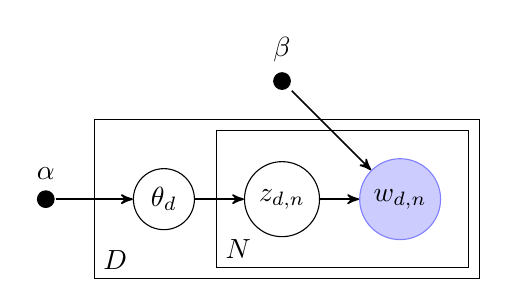
\begin{tikzpicture}
    [
      observed/.style={minimum size=15pt,circle,draw=blue!50,fill=blue!20},
      unobserved/.style={minimum size=15pt,circle,draw},
      hyper/.style={minimum size=1pt,circle,fill=black},
      post/.style={->,>=stealth',semithick},
    ]

    \node (w-j) [observed] at (0,0) {$w_{d,n}$};
    \node (z-j) [unobserved] at (-1.5,0) {$z_{d,n}$};
    \node (z-prior) [unobserved] at (-3,0) {$\theta_d$};
    \node (z-hyper) [label=above:$\alpha$] at (-4.5,0) {};
    \filldraw [black] (-4.5,0) circle (3pt);
    \node (w-hyper) [label=above:$\beta$] at (-1.5,1.5) {};
    \filldraw [black] (-1.5,1.5) circle (3pt);
    
    \path
    (z-j) edge [post] (w-j)
    
    (z-hyper) edge [post] (z-prior)
    (z-prior) edge [post] (z-j)

    (w-hyper) edge [post] (w-j)
    ;

    \node [draw,fit=(w-j) (z-prior), inner sep=14pt] (plate-context) {};
    \node [above right] at (plate-context.south west) {$D$};
    \node [draw,fit=(w-j) (z-j), inner sep=10pt] (plate-token) {};
    \node [above right] at (plate-token.south west) {$N$};

  \end{tikzpicture}
  \label{fig:lda-graphical-model}
\end{figure}

{$\theta_d$} represents the topic proportions for the \textit{d}th document
\\{$z_{d,n}$} represents the topic assignments for the \textit{n}th word in the \textit{d}th document
\\{$w_{d,n}$} represents the observed word for the \textit{n}th word in the \textit{d}th document
\\{$\beta$} represents a distribution over the words in the known vocabulary 

\begin{equation}\label{eq:KL}
KL(P\|Q) = \sum_i \ln\left(\frac{P(i)}{Q(i)}\right) P(i).\!
\end{equation}

\begin{equation}\label{eq:JS}
JS(P \parallel Q)= \frac{1}{2}KL(P \parallel M)+\frac{1}{2}KL(Q \parallel M), \hspace{0.2cm} where \hspace{0.2cm} M=\frac{1}{2}(P+Q)
\end{equation} 

\begin{equation}\label{eq:IR}
IR(P,Q) = 10^{-\beta{JS(P \parallel Q)}}
\end{equation}

\normalsize

	\note{Each review is a distribution over topics, so computing the similarity between two reviews translates to computing the similarity between their underlying topic distributions. The Kullback-Leibner (KL) measures the difference between two probability distributions \textit{P} and \textit{Q} as shown in equation. So it can be used to compute a value for the distance between the underlying topics distributions of two reviews. This measure has two drawbacks though. If \textit{Q(i)} is zero, then the measure is undefined. It is also not symmetric, meaning the divergence from \textit{P} to \textit{Q} is not the same as that from \textit{Q} to \textit{P}. Translating this to the reviews context, it is not a suitable metric to use, because if a review \textit{$R_1$} is similar to \textit{$R_2$} then it would be expected that \textit{$R_2$} is similar with the same amount to \textit{$R_1$}. 

The Jensen-Shannon (JS) measure is based on the KL divergence and it addresses these drawbacks: it is symmetric and always provides a finite value. It is also bounded by 1, which is more useful when comparing a similarity value for a review pair with a fixed threshold in order to classify the reviews as fake.

The JS measure can be rewritten, in order to decrease computational time for large vocabularies, as mentioned by Dagan et al.. IR is short for information radius, while {$\beta$} is a statistical control parameter.
	
}

}


\frame{
	\frametitle{Topics modeling for opinion spam detection}

	\setcounter{subfigure}{0}
	\begin{figure}
		\captionsetup[subfloat]{position=top,font=scriptsize,captionskip=-1.2pt}
		\begin{center}
			\subfloat[Subfigure 1 list of figures text][Precision]{
			\includegraphics[width=0.3\textwidth]{sweave/sweave-lda-precision}
			\label{fig:lda_precision}}
			\subfloat[Subfigure 2 list of figures text][Recall]{
			\includegraphics[width=0.3\textwidth]{sweave/sweave-lda-recall}
			\label{fig:lda_recall}}
			\subfloat[Subfigure 3 list of figures text][F1 Score]{
			\includegraphics[width=0.3\textwidth]{sweave/sweave-lda-f1score}
			\label{fig:lda_f1score}}
			\caption{Classifier results for the information radius similarity measure}    
			\label{fig:lda}
		\end{center}
	\end{figure}

	\begin{itemize}
		\item filtered out words that appeared  at most twice or more than 100 times
		\item when T > 0.7, P > 70\% ; P = 98\% for T = 0.95
		\item \#topics $\uparrow$ => performance $\downarrow$
		\item $P_{LDA}$ $\sim$ $P_{Mihalcea}$ for 30 and 50 topics
	\end{itemize}

	\note{I filtering out words that appeared either at most twice or more than 100 times in the review corpus. Although the distribution still has a positive skew, the filtering step has managed to improve the similarity results significantly, as it will be shown further on in this section. 

The original Blei LDA model was ran on a corpus made up of articles from Science magazine. These are relatively long English texts about various scientific themes, carefully edited to avoid misspelled words. It can be argued that the distribution tail of consumer reviews is longer than in the initial LDA model applied to edited scientific articles, since user reviews are short unedited texts, which can also contain misspelled words. Reviews are also not about varied themes, as the scientific articles, and tend to contain highly frequent words.
For 10 topics, the precision is more or less a flat line at 65\%. This could happen because 10 topics are way to little to summarize what people say about a seller. 
}

}

\frame{
	\frametitle{Wrap-up}	
	\begin{block}{Key points}
		\begin{itemize}
			\item shape of reviews in Trustpilot and Ott datasets => semantic similarity shows a more distinctive gap
			\item opinion spam detection using two new methods
			\item semantic similarity with WordNet => can outperform the vectorial-based measures
			\item topic modeling with LDA => performance $\sim$ vectorial models
			\item density clustering with DBSCAN and OPTICS on behavioral features
			\item comparison with cosine similarity and variations
			\item precision is good enough for production systems
		\end{itemize}
	\end{block}

}

\frame{
	\frametitle{}	

	\begin{center}
		\Huge
		\textbf{Questions?}
		\normalsize
	\end{center}

}
\end{document}